\documentclass{ctexart}
\usepackage{ctex}
\usepackage{graphicx}

\graphicspath{{figures/}}

\title{But How Do It Know}
\author{Mr Wu}
\date{\today}

\begin{document}
	\maketitle 
	5月13日开始,每天读半小时。
	\section{介绍}
	没什么好说的。
	\section{只有事实}
	这本书不是教科书,它的目的是为那些对计算机内部组成好奇的人解密计算机。
	
	这本书介绍了组成一台计算机所需要的全部条件。
	
	计算机领域有数以千计的名词和想法,但是其背后的基础概念是很简单的。
	
	这本书里没有任何东西需要记住。每一章介绍一个你没有听过的新的想法,或者是你曾经听过但仍然云里雾里的想法。每个想法都很简单,并且后面的想法建立在之前想法的基础上。
	\section{速度}
	计算机能够完成各种奇怪的事情,然而它们很简单。它们只能做很少,很简单的事情。它们看起来很复杂,是因为它们在很短的一段时间内做了很多简单的事情。
	
	计算机按顺序快速执行一些很简单的事情。当你了解了计算机的组成之后,你就会知道哪些事情计算机能做,哪些事情不能做。
	
	因此计算机的秘密不是它们有多复杂,而是它们的速度。让我们看看它们到底有多快!
	
	计算机基于电力工作,因此它们的速度和电力的速度有关。光速是186000里每秒,每秒可绕地球七圈。而电流在电线中的速度是光速的一半,每秒绕地球3.5圈。
	
	我们做一个比较:有一台电风扇在给你吹风,每秒40转,扇叶已经模糊。而电流的速度是每秒一亿转,很快。计算机每秒能做五亿件简单的事情。
	
	强调计算机到底有多快没什么意义。每隔一段时间,计算机厂商就会生产出速度两倍于之前的计算机。这个时间也就是摩尔定律表达的内容,摩尔定律:同面积的集成电路上可容纳的晶体管数量会以每年增加一倍的速度发展。具体的时间从一年变为两年,现在是三年。计算机的速度有一个理论上的极限值,关于这个极限,下面插入一段内容。
	\subsection{Extension--从工程方面讨论计算机的极限}
	2013年,摩尔定律被第二次修正,将之前每两年翻倍的发展速度改成了每三年翻倍。这次的修正从工程的角度来看至少有四个原因。
	
	首先是工艺的极限。现在的半导体制造工艺中很重要的一个部分是光刻(photolithography)。光刻利用曝光和显影在光刻胶层上画几何图形,然和通过刻蚀工艺(etching)将光掩膜上的图形转移到所在的衬底上。这种工艺在理论上受到阿贝分辨率的限制。简单地说,由于可见光的波动性使其可以发生衍射,光束不能无限的聚焦。而分辨率的极限值大约在λ?2n, 其中λ是光刻所用的激光波长,n是介质的数值孔径(Numerical Aperture)。数值孔径现在光学能达到的极限是1.4,那么光刻精度的极限就是λ?2.8。这么看来,要做到更小的工艺,我们就要用到波长更短的激光,而短波长的激光利用起来本就非常复杂。虽然科学家提出了新的工艺技术使得现在的光刻工艺突破了阿贝分辨率的限制,能够使用波长是193nm的激光能做出14nm的工艺,这种工艺技术也大大提高了制作成本。无论是在阿贝分辨率的限制下利用更短波长的激光还是开发出新技术来突破阿贝分辨率的限制,把单个晶体管做到更小(即在同面积的集成电路上容纳更多的晶体管)变得异常困难。
	
	其次是内部连接的极限。随着单位面积集成电路中的晶体管越来越多,内部连接成了集成电路中越来越重要的部分。内部连接要么做到快速的信号传输,要么做到尽量细的铜线和密集的排布(从而做到更小的集成电路设计),但鱼和熊掌不能可得兼。因为更细的铜线会增加铜线的电阻而更密集的排线也会影响铜线间电流的相互影响。早在1995年英特尔的研究员们就指出了真正限制集成电路发展的是其内部的连接技术 。为了解决这个问题,科学家们提出了光波导管(photonic waiveguide)的概念来替换传统的铜线连接方式 。而这种内部连接的方式也受到麦克斯维尔方程的理论限制,比如电磁波传输的速度上限。所以,即便是晶体管能够越做越小,如何在保证快速信号传输的同时加入更多的内部连接也成为了一个非常棘手的问题。
	
	再次是传统晶体管的设计极限。当晶体管尺寸做到10nm的时候,晶体管的栅氧化层仅仅之有几个原子的厚度。在这个尺度下至少会有三个问题。其一,在量子隧穿效应的影响下,晶体管的性质将变得很不稳定。其二,因为每个晶体管的制造过程不可能完全一样,每个晶体管会有不同的特性,而产生的不同特性在纳米级的尺度下会更加明显。其三,晶体管将会发生严重的漏电。这对移动设备兴起的今天是一个相当大的问题。毕竟谁也不希望自己的手机充电两小时,通话五分钟。因为量子效应在10nm左右的尺寸下介入,将传统晶体管做到这个尺度以下将会变得难上加难。当然科学家为了突破这个极限也提出了很多新的晶体管设计,其中比较成熟的有FinFET和 Tunneling Transistor。FinFET 在传统晶体管的基础上通过三维设计增加栅氧化层的宽度,而tuneling transistor 更是提出了控制量子隧穿的办法。但这些技术方面的改进也不是白来的,同样需要大量的资本投入,从而放缓了之前摩尔定律多设下的发展规则。
	
	最后一个要提到的是技术投入的极限。之前提到科学家们面临各种物理极限时候在晶体管制作工程方面提出的改变。而正是这些改变的措施造就了这第四项极限。新科技的研发需要大量的资金以及时间,即便是研发成功,公司的技术人员也需要投入大量的精力去学习并使用这些新的技术。这就导致了很多中小芯片制造商无力承担这项技术投入,而转向继续使用老技术进行生产加工。正是因为这些中小芯片厂商大量退出新技术的研发,芯片产业的发展在到达原有技术的理论极限之后遇到了发展的瓶颈。发展速度也因此明显放缓。这也是导致了2013年ITRS对摩尔定律进行了第二次的修正的原因之一。
	
	所以单纯将晶体管做小这条路不会一直走下去,而摩尔定律在今后的某个时间段可能会再一次遇到瓶颈。所以我们在30年后手拿天河2号的理想也不太可能实现。然而这一切似乎并不代表着结束,面对这一工程上面的限制,业界提出了一种新的发展方向——超越摩尔定律(More than Moore)。持有这个观念的计算机科学家们逐渐转向了对计算机体系结构的研究,更加侧重于功能的多样化,更多的靠电路设计及系统算法进行优化。于是,研究者们开始向更高维度来寻找可能性。就像当一个城市的道路无法满足人们的需求时就会出现地铁和高架桥,在二维工艺受限时,人们便开始探索三维集成电路。比如把处理器和内存上下堆叠,使用封装内走线来代替传统的二维平面走线做连接。这种三维结构不仅通过封装内走线的高密度性增加了内存访问带宽,同时也因为减少了连接长度而减少了数据访问的延迟。
	
	所以正如FinFET之父胡志明所说,“即便是面对如此之多的理论限制,半导体的发展并没有进入尾声,产业的进步需要我们通过不断的改进,过去五十年是这样走过来的,相信未来五十年也会这样走下去。”
	\subsection{Extension--Turing}
	计算机之父图灵是神一样的人物,是20世纪仅有的两个在智力上媲美爱因斯坦的人,另一位是冯.诺依曼。到底神在哪里?
	
	在计算机发展史上,常人的思路是工匠式的,也就是经过长期经验积累,从量变达到质变。图灵反其道而行之,20世纪20年代中期,图灵在思考三个问题:
	
	1.是否所有数学问题都有明确的答案?
	
	2.如果有,是否都能在有限步骤内计算出答案?
	
	3.对于那些有答案,且能在有限步骤之内计算出来的数学问题,能否设计一种机器,让它不断运转,当机器停下来时,就能解决该问题?
	
	所以图灵“神”在这里:一般人循序渐进地探索事物的发展规律,而图灵直接来到终点,并告诉大家,不要去做试图超越极限的事情。
	
	在上面的基础上,图灵进一步缩小了范围,也就是计算机能够在有限步骤内解决的问题。然后他设计了一种通用的方法,就是图灵机。下面用一张图总结人工智能的边界:
	
	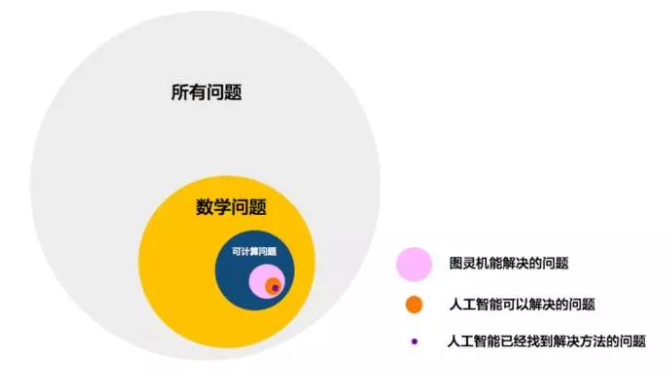
\includegraphics[scale=0.5]{1}
	
	图灵之所以能思考地如此深入,是受到了两个人的启发。
	
	第一位是数学大师希尔伯特。在1900年的巴黎国际数学家大会上,希尔伯特提出了23个重要的,根本的数学问题。其中第十个问题是:随便给一个不确定方程,能否通过有限步运算判断其是否存在整数解?如果答案是否定的,就说明很多问题连上帝都不知道答案是否存在。这个问题让图灵明白了计算机的极限所在。
	
	第二位是他的精神导师冯.诺依曼。图灵在拜读了冯.诺依曼的《量子力学的数学原理》之后,意识到计算来自于确定的机械运动。同时猜测人的意识来自于测不准原理,这是宇宙本身的规律。而计算是确定的,意识可以是不确定的。因此图灵得出结论:两者不可能相等。
	\subsection{Extension--从理论上计算未来电脑运算速度的极限}
	我们使用“终极笔记本电脑”来帮助计算,它的重量为1kg,体积为1L,并且在计算的物理极限下运行。当然,不考虑电池寿命。
	
	一、能量限制速度。这是相对论和量子力学的物理限制。
	
	爱因斯坦的质能方程是$ E = mc^2 $。海森堡的测不准原理表明,一个系统将至少花费一段时间来以某种可观察的方式改变,这段时间与系统的总能量有关。一个能量为E的系统,每秒可以执行$ 2E/\pi h $次逻辑运算。这里的$ h $是普朗克常数。普朗克常数记为h,是一个物理常数,用以描述量子大小。在量子力学中占有重要的角色,马克斯·普朗克在1900年研究物体热辐射的规律时发现,只有假定电磁波的发射和吸收不是连续的,而是一份一份地进行的,计算的结果才能和试验结果是相符。这样的一份能量叫做能量子,每一份能量子等于hν,ν为辐射电磁波的频率,h为一常量,叫为普朗克常数。在不确定性原理中 普朗克常数有重大地位,粒子位置的不确定性×粒子速度的不确定性×粒子质量≥普朗克常数。
	
	继续讨论。终极笔记本电脑的质量是1kg,因此能量$ E = mc^2 = 89874 \times 10^{16} J$,于是根据$ 2E/\pi h $计算出它每秒钟最多可以执行$ 5.4258 \times 10^{50} $次运算。而当前的计算速度离理论极限还有39个数量级的距离。
	
	二、熵限制内存。一个系统可以存储的数据量是它可以使用的可区分物理状态的数量的一个函数,因为每个不同的内存配置需要一个不同的物理状态。系统的热力学熵如下表示:$ S =  K_{B}logW$,其中$ K_{B} $是玻尔兹曼常数,$ W $是系统中的状态数目。所以,如果我们知道系统的熵,就可以计算出终极笔记本电脑可以计算出的比特数。
	
	然而计算系统的精确熵及其困难。最终的结果是,在最大熵下运行的终极笔记本电脑,可以存储至少$ 2.13 \times 10^{31} $比特。当然,最大熵意味着笔记本电脑的所有物质都转化为能量,基本上等同于热核爆炸。
	
	现代计算机有多接近这个极限?在2008年,一台现代的笔记本电脑可以存储250GB,大约$ 2 \times 10^{12} $位。距离最大存储容量大约还有19个数量级,或者说是容量再翻倍64次。从1956年到2005年,每平方英寸的磁盘容量已经翻倍了30次。按照这个历史速度,磁盘容量的64次翻倍将只需要大约50到100年的时间。这并不是摩尔定律在计算上的总体限制,但是它暗示了在我们有生之年可以结束摩尔定律的应用的可能性。
	
	三、终极笔记本电脑的影响。计算终极笔记本电脑的极限确实是很有趣的,但是这对今天的计算机科学又意味着什么呢?我们现在已经可以推导出一个理论上的上限,来解释广义摩尔定律能够持续多久。目前的笔记本电脑存储$ 10^{12} $位,每秒处理$ 10^{12} $个单位操作。终极笔记本电脑可以存储$ 10^{31} $位数据,每秒处理$ 10^{51} $个单位运算,这分别相差了$ 10^{19} $和$ 10^{39} $个数量级。劳埃德估计,在过去的50年里,摩尔定律的比率的提升是108个数量级。假设存储密度和计算速度都会每50年提高108倍,那么存储容量将在大约125年内达到极限,而每秒钟的运算速度将在250年内达到极限。有人认为,在最后的125年里,人们会疯狂地开发更好的压缩算法——或者是更先进的理论物理学。
	
	一旦摩尔定律停止,想要提升计算能力的方法就只能是增加计算机的质量和体积,但这也会遇到基本的限制。根据一篇题为《计算的普遍限制》的未发表的论文估计,根据摩尔定律,整个宇宙的计算能力将在600年后耗尽。
	
	50年的时间是一段迷人的时光。它看似与今天活着的人联系非常遥远,但事实上已经足够近了,我们完全做不到忽视它。人类长期活动的典型规划范围(比如管理生态系统)大约有300年的历史,因此为摩尔定律的终结进行规划也是说得通的。
	\subsection{EEExtension}
	讲到这里,又要插入一段题外话。上文中提到,常人是工匠式思路,而图灵直接来到了终点。表面上看,图灵是受到了希尔伯特的启发。然而如果继续探究,会发现事实远比这复杂。详情可以参考下面这篇文章:
	
	http://mindhacks.cn/2006/10/15/cantor-godel-turing-an-eternal-golden-diagonal/
	
	要想搞清楚图灵机的来龙去脉,我们得从第三次数学危机说起。既然有第三次,就有前面两次。为了保持连续性,我们从第一次数学危机开始,追根溯源。
	\subsubsection{第一次数学危机}
	古希腊有一位著名的数学家--毕达哥拉斯。他的主要观点是万物皆整数,即万物都可以用整数来表示。具体来说,一个数要么是整数,要么是两个整数的比值。毕达哥拉斯又提出了勾股定理,也就是直角三角形斜边的平方等于另外两条边的平方和。它的一个学生希帕索斯发现了一个问题:如果两条直角边都是1,那么斜边是多少?答案是$ \sqrt{2} $。$ \sqrt{2} $是一个无理数,不能用任何两个整数的比值来表示,毕达哥拉斯自己也无法解释,这就是第一次数学危机。另外,既然解释不了,就要掩饰,于是他把希帕索斯扔进了爱琴海。因此他成了历史上第一位学术界的恶棍--学霸。
		那么第一次危机是如何解决的呢?约在公元前370年,柏拉图的学生攸多克萨斯解决了关于无理数的问题。他纯粹用公理化方法创立了新的比例理论,微妙地
	处理了可公度和不可公度。
	\subsubsection{第二次数学危机}
	第二次数学危机质疑的是微积分的基础问题。微积分中的导数定义为$ lim_{\Delta x \to 0}\frac{\Delta y}{\Delta x} $。直到1734年,英国的大主教贝克莱提出了一个问题:无穷小到底是不是零?如果是零,它就不能作为分母;如果不是零,也会导致矛盾。牛顿,莱布尼茨等人都设法解释这个微积分基础的不严密性的问题,但没有成功。
	
	直到19世纪70年代,柯西,康托尔等人在实数理论的基础上建立起极限理论,第二次危机才算是彻底解决。
	\subsubsection{第三次数学危机}
	第三次数学危机始于罗素提出的“理发师悖论”:在一个村子里,一个理发师只给不给自己刮胡子的人刮胡子。那么这个理发师给自己刮胡子吗?罗素提出的这个问题是对康托尔集合论的质疑,也就是集合的自我指涉问题。康托尔面对质疑无法解释,郁郁而终。事实上直至今日,第三次数学危机也没有得到解决。
	
	那么第三次数学危机和图灵机有什么关系?上文说到,1900年希尔伯特提出了23个数学问题,这23个问题汇总到一起,实际上是想构建一个数学体系。首先定义一批公理和基本逻辑规则,然后依据这些公理和逻辑规则可以推演出这个体系内的无穷多的定理——这就应该是理想的数学。
	
	要理解这个体系的概念,需要先理解形式系统。一个形式系统必须满足四个性质。首先是有效性,即如果前提为真,推导出来的结论也是真的。第二条是可靠性,即系统中所有的定理皆为真。第三条是自洽性,即系统内任意两个真命题不能互相矛盾。这个性质也叫做无矛盾性或相容性。最后一条是完备性,即系统中任何一个命题都是可证明或可证伪的。
	
	在此基础上,希尔伯特的思考上升了一个层次。数学里包含各个分支,如果把数学的所有研究内容看做一个系统,各个分支为子系统,那么整个数学是上述的形式系统吗?如果是,那么数学中所有的命题都可被证明或者被证伪。也就是说,没有我们不知道的事情,只有我们还没能知道的事情。这也是希尔伯特的墓志铭:我们必须知道,我们必将知道。
	
	遗憾的是,这个问题的答案是否定的。给出这个答案的人是哥德尔,他提出了哥德尔不完备定理。
	
	哥德尔不完备定理是数理逻辑学中论述形式公理化系统局限性的两条重要定理。哥德尔写道:“众所周知,数学朝着更为精确方向的发展,已经导致大部分数学分支的形式化,以致人们只用少数几个机械规则就能证明任何定理。因此人们可能猜测这些公理和推理规则足以决定这些形式系统能加以表达的任何数学问题。下面将证明情况并非如此。”
	
	哥德尔不完备定理一:任何一个包含自然数公理的公理体系,如果它是相容的,则它不是完备的。也就是说,一个相容的形式系统中,必然存在一个命题,它既不能被证明,也不能被证伪。证明过程是这样的:在形式系统T中,哥德尔构造了一个命题P:P不可在系统T内被证明。如果P为假,也就是P可以在系统T内被证明,那么系统T推出了一个假命题,这违反了可靠性。因此P为真,但这又推出P不可在系统T内被证明,这违反了完备性。
	
	至此,证明的关键变成了这个问题:在系统T中能构造出这个命题吗?如果能,该怎么构造?这个问题的解决是哥德尔编码,具体就不说了,太过高深。总之,这个命题P是可以构造出来的。于是得到哥德尔第一不完备定理:一个自洽的系统一定不是完备的。
	
	哥德尔第二不完备定理:形式系统的一致性无法在系统内得到证明。一致性也就是无矛盾性,即系统不会推出互相矛盾的命题。
	
	到这里,终于与图灵机联系起来了。可以认为图灵机和哥德尔不完备定理是等价的。最后,哥德尔不完备定理的意义:
	
	一、哥德尔不完备性定理深刻地揭示了形式系统的内在局限性。这种局限性是由形式系统的本质所决定的,是不可克服的。因为一个形式体系的无矛盾性在本质上是超越这个形式体系的。它处在一种两难境地:或者允许在逻辑思维中有矛盾存在,或者承认存在着逻辑方法证明不了的本逻辑系统内部的问题。因此,那种希望把数学搞成一个形式化系统,希望所有的猜想都能从逻辑出发加以判定,希望永远不发生出乎始料的事,是不可能实现的。数学不等于逻辑,重要的数学成果并不总是能从公理直接逻辑地推出,数学的神奇之处主要扎根于观察、直觉和灵感。
	
	事实上,不论是作为科学认识前提的公理、假设,还是在一定前提下的逻辑推理,都有其预设的不可证明的信念。人类认识世界总在定的信念指导下的逻辑展开,并在获得新知识的过程中不断扩展着对世界新的观念。因此,信念的合理性是相对的,它要随着认识的深化而不断发展变化。在信念转化为知识的过程中,真正起作用的是科学家的非机械的、非逻辑的智力创造,逻辑的一致性只是一种理想的指向和要求。
	
	二、哥德尔不完备性定理也进一步揭示了人工智能系统的局限性,从本质上证明了机械论、还原论是错误的。按照他们的观点,精神活动过程同机器执行程序一样,不过是在从事某种良定义的被称为算法"的运算过程,而人脑和简单的计算机的主要差别仅仅在于人脑活动具有更大的复杂性,或者表现为更高级的结构,人的所有精神品质,包括思维、情感、智慧、意识都不过是大脑执行的算法特征而已。
	
	但是,人脑终究不能解释成机器,计算机绝不可能超越人类心智。因为,无论我们构造出多么复杂的机器,只要它是机器,就将对应于一个形式系统,就能找到一个在该系统内不可证的公式而使之受到哥德尔理论的打击,机器不能把这个公式作为定理推导出来,但是人心却能看出它是真的。因此这台机器不是心的一个恰当模型。我们总想制造心的一种机械模型,即从本质上是死的模型,而心是活的,它总能比任何形式的、僵死的系统干得更好。这也诚如英国数学家、物理学家罗杰·彭罗斯所说,人类判断数学真理的过程是超越任何算法的,因为,意识是我们赖以理解数学真理的关键,这种意识是我们能够借直觉的洞察力看出某些在数学形式系统中不能证明的数学命题的真理性,而意识是不能被形式化的,它必定是非算法的。因此,计算机不过是强人工智能专家所钟爱的一副"皇帝新脑"而已。
	
	三、数学是科学的基础,数学的不完备性说明科学结论也是不完备的。自从近代科学开始自然的数学化努力以来,科学问题就是被数学编码的问题,科学结论就是被数学化的结论。正是由于作为科学的语言、模式、方法和工具的数学本身的不完备性,导致了由它所表述、绘制的科学结论的不完备性。科学结论的不完备性具有重大的科学价值。科学结论的不完备性预示着存在着许多不可解的科学问题或否定性的科学结论,从而产生了大批限制性成果。如,计算机与人工智能之父图灵证明没有一个程序能够证明检验任何程序是否将在某个时候停止(即停机问题)。
	
	科学结论的不完备性还有着独特的哲学意义。正如我国著名科学家郝柏林院士所言,"否定比肯定更具普遍性"。在科学上,一个否定性结论的形成往往标志着一个新科学方向的产生。认识到绝对温度零度不能达到,恰恰是低温物理学的开始;认识到质点不能超光速运动,正好是相对论的开端;认识到测不准原理,恰好是量子力学的诞生,如今,又是由于不确定性、不可预测性现象的发现,一门全新的复杂性科学正在蓬勃兴起。
	
	四、哥德尔不完备性定理从科学的层次上揭示了人类认识的局限性。在回答有关自然和人类社会的问题上,许多人似乎从来就没有经过认真地思考便不由自主地接受了人的心智或认知能力是没有根本性限制的观点。但是,自己的创造物正是反观自己的最好镜面,数学作为人类心智与理性的产物,正好反观了人类认知的局限性或不完备性。形式系统的不完备性必然根源于它的创造者的不完备性。
	
	人类心智与理性的不完备性也是基于人类及其心智和理性均是生物进化的产物这一基本认识的必然推断。只要人们承认这一进化论的结论,那么就不难认识到,人类的心智与理性是受制于进化水平的。也就是说,人类进化到什么程度,其心智与理性使达到什么水准,它们是处在一个不断进化的过程之中的,它们本身就是人类生命的一个有机组成部分。这样来,任何一个特定历史阶段,人的心智与理性水准都是有限的,它不可能穷尽无限,达到全知。心理与理性的这种有限性或局限性,必然通过自己的不完备的创造物得以显现。
	\subsubsection{The Last Extension--NP Problem}
	P问题是多项式时间内可以解决的问题,NP问题是多项式时间内可以验证的问题。显然,P问题一定属于NP问题。那么,P问题=NP问题?
	
	这个问题暂时没有解决,但是有一点进步。我们知道,如果一个问题A可以约化到问题B,而B问题是P问题,那么A问题也就解决了。那么,是否所有的NP问题都可以约化到某一类问题,只要解决了这一类问题,就能解决NP问题呢?答案是肯定的,这一类问题就是NPC问题。NPC问题的定义:首先它是NP问题,其次,所有的NP问题都可以在多项式时间内约化到它。于是,只要我们能在多项式时间内解决一个NPC问题,就等于在多项式时间内解决了所有NP问题,于是推出P问题=NP问题。
	
	所以最后问题的关键是,能不能在多项式时间内解决任意一个NPC问题?目前还没有找到这样的NPC问题。
	\section{语言}
	
\end{document}